\documentclass[12pt,a4paper]{article}

%=========
% PACKAGES
%=========

\usepackage{graphicx}
\usepackage[section]{placeins}
\usepackage{float}
\usepackage{amsmath}
\usepackage{listings}
\usepackage{xcolor}
\usepackage{extarrows}
\usepackage{verbatim}
\usepackage{enumerate}
\usepackage{enumitem}
\usepackage{eurosym}
\usepackage{svg}
\usepackage{varwidth}
\usepackage{moreverb}
\usepackage{relsize}
\usepackage{tabto}
\usepackage[margin=1in]{geometry}
\usepackage[normalem]{ulem}
\usepackage{units}
\usepackage{fancyvrb}
\usepackage{fontspec}
\usepackage{extarrows}
\usepackage{amsfonts}
\usepackage{amssymb}
\usepackage{hyperref}
%\usepackage{unicode-math}


%=====================
% SETTINGS/DEFINITIONS
%=====================

% Don't break words with hyphens. Instead, wrap word to next line.
\tolerance=1
% \emergencystretch=\maxdimen
\hyphenpenalty=10000
\hbadness=10000

\definecolor{codegreen}{rgb}{0,0.6,0}
\definecolor{codegray}{rgb}{0.5,0.5,0.5}
\definecolor{codepurple}{rgb}{0.58,0,0.82}
\definecolor{backcolour}{rgb}{0.95,0.95,0.92}

\def\verbatimtabsize{4}

\lstdefinestyle{mystyle}{
	backgroundcolor=\color{backcolour},
	commentstyle=\color{codegreen},
	keywordstyle=\color{magenta},
	numberstyle=\tiny\color{codegray},
	stringstyle=\color{codepurple},
	basicstyle=\ttfamily\footnotesize,
	breakatwhitespace=false,
	breaklines=true,
	captionpos=b,
	keepspaces=true,
	numbers=left,
	numbersep=5pt,
	showspaces=false,
	showstringspaces=false,
	showtabs=false,
	tabsize=2
}

\lstset{style=mystyle}

\setlength{\parindent}{0pt}
\setlength{\parskip}{0em}
\setlength{\jot}{4mm}

\pagenumbering{gobble}

\hypersetup{
    colorlinks=true,
    linkcolor=blue,
    filecolor=blue,      
    urlcolor=blue,
}

\setmainfont{Minion Pro}

\newcommand{\imagesPath}{/home/nick/shmmy/8th/slp/slp-ntua/set2}

\title{Επεξεργασία Φωνής και Φυσικής Γλώσσας \\ 2η σειρά αναλυτικών ασκήσεων}
\author{Νικόλαος Παγώνας, el18175}
\date{}

\begin{document}
	\maketitle	
	
	\section*{Άσκηση 1} 
		
		\subsection*{1.}
			Έχουμε:
			
			\begin{align*}
				E_x &= \sum_{n=0}^{N-1+p}\left(e^2\left(n\right)\right) \\ 
					&= \sum_{n=0}^{N-1+p}\left(\sum_{k=0}^{p}a_{xk}x\left(n-k\right)\right)^2 \\ 
					&= \sum_{n=0}^{N-1+p}\left(\sum_{k=0}^{p}a_{xk}x\left(n-k\right)\right)\left(\sum_{\ell=0}^{p}a_{x\ell}x\left(n-\ell\right)\right) \\ 
					&= \sum_{k=0}^{p}a_{xk}\sum_{\ell=0}^{p}a_{x\ell}\sum_{n=0}^{N-1+p}x\left(n-k\right)x\left(n-\ell\right) 
			\end{align*}
			
			Και επειδή:
			
			\begin{align*}
				\sum_{n=0}^{N-1+p}x\left(n-k\right)x\left(n-\ell\right) = \sum_{n=0}^{N-1+p}x\left(n\right)x\left(n-\ell+k\right)=R_x\left(k-\ell\right)
			\end{align*}
			
			Προκύπτει ότι:
			
			\begin{align*}
				E_x &= \sum_{k=0}^{p}a_{xk} \sum_{\ell=0}^{p}a_{x\ell}R_x\left(k-\ell\right) \\
				&= a_xR_xa_x^T
			\end{align*}
			
			όπου:
			
			\[
				R = \begin{bmatrix}
					R_x\left(0\right) & R_x\left(1\right) & \dots & R_x\left(p\right) \\
					R_x\left(1\right) & R_x\left(0\right) & \dots & R_x\left(p-1\right) \\
					\vdots & & \ddots \\
					R_x\left(p\right) & R_x\left(p-1\right) & \dots & R_x\left(0\right)
				\end{bmatrix}  \text{, διάστασης (p+1)$\times$(p+1)}
			\]
			
		\subsection*{2.}
			Έχουμε:
			
			\begin{align*}
				E_{xy} &= \sum_{n=0}^{N-1+p} \left(\sum_{k=0}^{p}a_{yk}x\left(n-k\right)\right)^2 \\
				&= \sum_{n=0}^{N-1+p}\left(\sum_{k=0}^{p}a_{yk}x\left(n-k\right)\right)\left(\sum_{\ell=0}^{p}a_{y\ell}x\left(n-\ell\right)\right) \\
				&= \sum_{k=0}^{p}a_{yk}\sum_{\ell=0}^{p}a_{y\ell}\sum_{n=0}^{N-1+p}x\left(n-k\right)x\left(n-\ell\right) \\
				&= \sum_{k=0}^{p}a_{yk}\sum_{\ell=0}^{p}a_{y\ell}R_x\left(k-\ell\right) \\
				&= a_yR_xa_y^T
			\end{align*}
			
			όπου $R_x$ ο πίνακας του προηγούμενου ερωτήματος.
		
		\subsection*{3.}
			Καταρχάς, για το $x\left(n\right)$ οι βέλτιστοι LPC συντελεστές είναι $a_x = \left(a_{x0}, \dots, a_{xp}\right)$, οπότε η $E_x$ είναι η ελάχιστη δυνατή για γραμμική πρόβλεψη με τους συντελεστές $a_x$. Επομένως, αν κάνουμε γραμμική πρόβλεψη του $x\left(n\right)$ με τους συντελεστές του $y\left(n\right)$, τότε η ενέργεια του σφάλματος πρόβλεψης $E_{xy}$ θα είναι σίγουρα μεγαλύτερη ή ίση της $E_x$:
			
			\begin{align*}
				\dfrac{E_{xy}}{E_x} \geq 1.
			\end{align*}
	
	\section*{Άσκηση 2} 
		
		\subsection*{1.}
			Έχουμε:
			
			\begin{align*}
				\delta_t\left(i\right) &= \max_{q_1, \dots, q_{t-1}} P\left[q_1...q_{t-1}, q_t=i, O_1...O_t|\lambda\right] \\
				&= \max_{q_1, \dots, q_{t-1}} \{P\left(q_1\right)P\left(q_2|q_1\right) \dots P\left(q_t=i|q_{t-1}\right)P\left(O_1|q_1\right)\dots P\left(O_t|q_t\right)\} \\
				&= \max_{q_1, \dots, q_{t-1}} \{\pi_1 a_{12} a_{23} \dots P\left(q_t=i|q_{t-1}\right)b_{q1}\left(O_1\right)\dots b_{q_t}\left(O_t\right)\} \\
				&= b_{q_t}\left(O_t\right)\max_{q_{t-1}}\{b_{q_{t-1}}\left(O_{t-1}\right)P\left(q_t=i|q_{t-1}\right)\max_{q_{t-2}}\{\dots \max_{q_2}\{b_{q_2}\left(O_2\right)a_{23}\max_{q_1}\{b_{q_1}\left(O_1\right)a_{12}\pi_1\}\}\}\}
			\end{align*}
			
			Χρησιμοποιούμε τον αλγόριθμο Viterbi:
			
			\subsubsection*{(i) Αρχικοποίηση}
				\begin{align*}
					\delta_1\left(i\right) &= \pi_1 b_i\left(O_1\right)  ~~~~~\left(O_1 = U\right)
				\end{align*}
				
				\begin{align*}
					\delta_1\left(1\right) = 0.1, ~
					\delta_1\left(2\right) = 0.075, ~
					\boxed{\delta_1\left(3\right) = 0.2}, ~
					\delta_1\left(4\right) = 0.188   
				\end{align*}
				
			\subsubsection*{(ii) Επανάληψη} 
				\begin{align*}
					\delta_{t+1}\left(j\right) = \left(\max_{i}\delta_t\left(i\right)a_{ij}\right)\cdot b_j\left(O_{t+1}\right)
				\end{align*}
			
				\begin{itemize}
					\item $t=2, ~ O_2=V$
					\begin{align*}
						\delta_2\left(1\right) = 36\times10^{-3}, ~
						\boxed{\delta_2\left(2\right) = 39.4\times10^{-3}}, ~
						\delta_2\left(3\right) = 9.38\times10^{-3}, ~
						\delta_2\left(4\right) = 15\times10^{-3}
					\end{align*}
					
					\item $t=3, ~ O_3=U$
					\begin{align*}
						\delta_3\left(1\right) = 4.73\times10^{-3}, ~
						\delta_3\left(2\right) = 3.24\times10^{-3}, ~
						\boxed{\delta_3\left(3\right) = 9.45\times10^{-3}}, ~
						\delta_3\left(4\right) = 7.38\times10^{-3}
					\end{align*}

					\item $t=4, ~ O_4=V$
					\begin{align*}
						\boxed{\delta_4\left(1\right) = 17\times10^{-4}}, ~
						\delta_4\left(2\right) = 16.5\times10^{-4}, ~
						\delta_4\left(3\right) = 3.69\times10^{-4}, ~
						\delta_4\left(4\right) = 7.09\times10^{-4}
					\end{align*}
					\item $t=5, ~ O_5=V$
					\begin{align*}
						\delta_5\left(1\right) = 2.98\times10^{-4}, ~
						\boxed{\delta_5\left(2\right) = 3.57\times10^{-4}}, ~
						\delta_5\left(3\right) = 1.02\times10^{-4}, ~
						\delta_5\left(4\right) = 1.06\times10^{-4}
					\end{align*}
					
					\item $t=6, ~ O_6=U$
					\begin{align*}
						\delta_6\left(1\right) = 4.29\times 10^{-5}, ~
						\delta_6\left(2\right) = 2.68\times 10^{-5}, ~
						\boxed{\delta_6\left(3\right) = 8.57\times 10^{-5}}, ~
						\delta_6\left(4\right) = 6.7\times 10^{-5}
					\end{align*}
					
					\item $t=7, ~ O_7=V$
					\begin{align*}
						\boxed{\delta_7\left(1\right) = 15.4\times10^{-6}}, ~
						\delta_7\left(2\right) = 15\times10^{-6}, ~
						\delta_7\left(3\right) = 3.35\times10^{-6}, ~
						\delta_7\left(4\right) = 6.43\times10^{-6}
					\end{align*}
					
					\item $t=8, ~ O_8=U$
					\begin{align*}
						\delta_8\left(1\right) = 1.8\times10^{-6}, ~
						\delta_8\left(2\right) = 1.39\times10^{-6}, ~
						\boxed{\delta_8\left(3\right) = 3.7\times10^{-6}}, ~
						\delta_8\left(4\right) = 2.89\times10^{-6}
					\end{align*}

					\item $t=9, ~ O_9=V$
					\begin{align*}
						\boxed{\delta_9\left(1\right) = 6.67\times10^{-7}}, ~
						\delta_9\left(2\right) = 6.48\times10^{-7}, ~
						\delta_9\left(3\right) = 1.45\times10^{-7}, ~
						\delta_9\left(4\right) = 2.78\times10^{-7}
					\end{align*}

					\item $t=10, ~ O_{10}=U$
					\begin{align*}
						\delta_{10}\left(1\right) = 7.78\times10^{-8}, ~
						\delta_{10}\left(2\right) = 6\times10^{-8}, ~
						\boxed{\delta_{10}\left(3\right) = 16\times10^{-8}}, ~
						\delta_{10}\left(4\right) = 12.5\times10^{-8}
					\end{align*}
				\end{itemize}
		
		\subsection*{2.}
			Σύμφωνα με τον παραπάνω αλγόριθμο, η πιθανότερη ακολουθία καταστάσεων είναι: \\
			
			\[
				Q^*: 3\rightarrow2\rightarrow3\rightarrow1\rightarrow2\rightarrow3\rightarrow1\rightarrow3\rightarrow1\rightarrow3
			\]
		
		\subsection*{3.}
			Είναι:
			
			\begin{align*}
				P^* = (\textbf{O}, \textbf{Q}^*|\lambda) = \delta_{10}(3) = 16 \times 10^{-8}
			\end{align*}
	
	\section*{Άσκηση 3} 
		
		\subsection*{1.}
			Δίνεται το ακόλουθο φωνητικό λεξικό:
			
			\begin{verbatim}
				any          eh n iy
				e.           iy
				many         m eh n iy
				men          m eh n
				per          p er
				persons      p er s uh n z
				sons         s uh n z
				suns         s uh n z
				to           t uw
				tomb         t uw m
				too          t uw
				two          t uw
			\end{verbatim}
		
		\subsection*{2.}
			Ακολουθούμε μία διαδικασία ανάλογη του 1ου εργαστηρίου. Αρχικά, δημιουργούμε το \verb|phones.syms|:
			
			\begin{verbatim}
				<eps> 0
				eh 1
				er 2
				iy 3
				m 4
				n 5
				p 6
				s 7
				t 8
				uh 9
				uw 10
				z 11
			\end{verbatim}
			
			Ύστερα δημιουργούμε την μηχανή πεπερασμένης κατάστασης που υλοποιεί την απόσταση που περιγράφεται στην εκφώνηση της άσκησης. \href{https://imgur.com/a/S3IAVKw}{Η απεικόνιση της μηχανής πεπερασμένης κατάστασης βρίσκεται εδώ.} Ύστερα, με χρήση των script \verb|word_edits.sh| και \verb|mkfstinput.py| δημιουργούμε αποδοχείς για τις λέξεις (φώνημα-φώνημα), οπότε μπορούμε να υπολογίσουμε την ελάχιστη φωνολογική απόσταση ανάμεσα σε δύο λέξεις του λεξικού. Έτσι, έχουμε:
			
			\begin{verbatim}
any --> any
======================

any --> e
======================
eh <eps> 1.20000005
n <eps> 1.20000005

any --> many
======================
<eps> m 1.20000005

any --> men
======================
<eps> m 1.20000005
iy <eps> 1.20000005

any --> per
======================
eh <eps> 1.20000005
iy er 1
n p 1

any --> persons
======================
<eps> p 1.20000005
iy z 1
<eps> uh 1.20000005
<eps> s 1.20000005
eh er 0.5

any --> sons
======================
<eps> s 1.20000005
iy z 1
eh uh 1

any --> suns
======================
<eps> s 1.20000005
iy z 1
eh uh 1

any --> to
======================
eh <eps> 1.20000005
iy uw 1
n t 1

any --> tomb
======================
eh t 1
iy m 1
n uw 1

any --> too
======================
eh <eps> 1.20000005
iy uw 1
n t 1

any --> two
======================
eh <eps> 1.20000005
iy uw 1
n t 1

e --> e
======================

e --> many
======================
<eps> m 1.20000005
<eps> n 1.20000005
<eps> eh 1.20000005

e --> men
======================
iy m 1
<eps> n 1.20000005
<eps> eh 1.20000005

e --> per
======================
iy p 1
<eps> er 1.20000005

e --> persons
======================
iy p 1
<eps> z 1.20000005
<eps> n 1.20000005
<eps> uh 1.20000005
<eps> s 1.20000005
<eps> er 1.20000005

e --> sons
======================
iy s 1
<eps> z 1.20000005
<eps> n 1.20000005
<eps> uh 1.20000005

e --> suns
======================
iy s 1
<eps> z 1.20000005
<eps> n 1.20000005
<eps> uh 1.20000005

e --> to
======================
iy t 1
<eps> uw 1.20000005

e --> tomb
======================
iy t 1
<eps> m 1.20000005
<eps> uw 1.20000005

e --> too
======================
iy t 1
<eps> uw 1.20000005

e --> two
======================
iy t 1
<eps> uw 1.20000005

many --> many
======================

many --> men
======================
iy <eps> 1.20000005

many --> per
======================
m p 1
iy <eps> 1.20000005
n <eps> 1.20000005
eh er 0.5

many --> persons
======================
m p 1
iy z 1
<eps> uh 1.20000005
<eps> s 1.20000005
eh er 0.5

many --> sons
======================
m s 1
iy z 1
eh uh 1

many --> suns
======================
m s 1
iy z 1
eh uh 1

many --> to
======================
m <eps> 1.20000005
iy uw 1
n t 1
eh <eps> 1.20000005

many --> tomb
======================
m t 1
iy <eps> 1.20000005
n m 0.5
eh uw 1

many --> too
======================
m <eps> 1.20000005
iy uw 1
n t 1
eh <eps> 1.20000005

many --> two
======================
m <eps> 1.20000005
iy uw 1
n t 1
eh <eps> 1.20000005

men --> men
======================

men --> per
======================
m p 1
n <eps> 1.20000005
eh er 0.5

men --> persons
======================
m p 1
<eps> z 1.20000005
<eps> uh 1.20000005
<eps> s 1.20000005
eh er 0.5

men --> sons
======================
m s 1
<eps> z 1.20000005
eh uh 1

men --> suns
======================
m s 1
<eps> z 1.20000005
eh uh 1

men --> to
======================
m <eps> 1.20000005
n uw 1
eh t 1

men --> tomb
======================
m t 1
n m 0.5
eh uw 1

men --> too
======================
m <eps> 1.20000005
n uw 1
eh t 1

men --> two
======================
m <eps> 1.20000005
n uw 1
eh t 1

per --> per
======================

per --> persons
======================
<eps> z 1.20000005
<eps> n 1.20000005
<eps> uh 1.20000005
<eps> s 1.20000005

per --> sons
======================
p s 1
<eps> z 1.20000005
<eps> n 1.20000005
er uh 1

per --> suns
======================
p s 1
<eps> z 1.20000005
<eps> n 1.20000005
er uh 1

per --> to
======================
p t 0.5
er uw 1

per --> tomb
======================
p t 0.5
<eps> m 1.20000005
er uw 1

per --> too
======================
p t 0.5
er uw 1

per --> two
======================
p t 0.5
er uw 1

persons --> persons
======================

persons --> sons
======================
p <eps> 1.20000005
er <eps> 1.20000005

persons --> suns
======================
p <eps> 1.20000005
er <eps> 1.20000005

persons --> to
======================
p t 0.5
z <eps> 1.20000005
n <eps> 1.20000005
uh uw 0.5
s <eps> 1.20000005
er <eps> 1.20000005

persons --> tomb
======================
p t 0.5
z <eps> 1.20000005
n m 0.5
uh uw 0.5
s <eps> 1.20000005
er <eps> 1.20000005

persons --> too
======================
p t 0.5
z <eps> 1.20000005
n <eps> 1.20000005
uh uw 0.5
s <eps> 1.20000005
er <eps> 1.20000005

persons --> two
======================
p t 0.5
z <eps> 1.20000005
n <eps> 1.20000005
uh uw 0.5
s <eps> 1.20000005
er <eps> 1.20000005

sons --> sons
======================

sons --> suns
======================

sons --> to
======================
s t 1
z <eps> 1.20000005
n <eps> 1.20000005
uh uw 0.5

sons --> tomb
======================
s t 1
z <eps> 1.20000005
n m 0.5
uh uw 0.5

sons --> too
======================
s t 1
z <eps> 1.20000005
n <eps> 1.20000005
uh uw 0.5

sons --> two
======================
s t 1
z <eps> 1.20000005
n <eps> 1.20000005
uh uw 0.5

suns --> suns
======================

suns --> to
======================
s t 1
z <eps> 1.20000005
n <eps> 1.20000005
uh uw 0.5

suns --> tomb
======================
s t 1
z <eps> 1.20000005
n m 0.5
uh uw 0.5

suns --> too
======================
s t 1
z <eps> 1.20000005
n <eps> 1.20000005
uh uw 0.5

suns --> two
======================
s t 1
z <eps> 1.20000005
n <eps> 1.20000005
uh uw 0.5

to --> to
======================

to --> tomb
======================
<eps> m 1.20000005

to --> too
======================

to --> two
======================

tomb --> tomb
======================

tomb --> too
======================
m <eps> 1.20000005

tomb --> two
======================
m <eps> 1.20000005

too --> too
======================

too --> two
======================

two --> two
======================
			\end{verbatim}
			
	
	\section*{Άσκηση 4} 
		Δίνεται το ακόλουθο φωνητικό λεξικό:
		
		\begin{verbatim}
			any                  eh n iy
			e.                   iy
			many                 m eh n iy
			men                  m eh n
			per                  p er
			persons              p er s uh n z
			lessons              l eh s uh n z
			sons                 s uh n z
			suns                 s uh n z
			sunset               s uh n z eh t
			to                   t uw
			tomb                 t uw m
			too                  t uw
			two                  t uw
		\end{verbatim}
		
		\subsection*{1.}
			Σχεδιάζουμε τον μετατροπέα που αντιστοιχίζει σειρές από φωνήματα σε λέξεις:
			
			\begin{figure}[H]
				\begin{center}
					\includegraphics[width=\linewidth]{\imagesPath/ex4/L.pdf}
				\end{center}
			\end{figure}
		
		\subsection*{2.}
			
		
		\subsection*{3.}
			
	
	\section*{Άσκηση 5} 
		
		\subsection*{1.}
		
			\subsubsection*{(a)}
				Μπορούμε να θεωρήσουμε ότι τα δεδομένα που δίνονται στην εκφώνηση αποτελούνται μόνο από δισύλλαβες λέξεις, αφού οι λέξεις με μία συλλαβή εμφανίζονται εξίσου συχνά με τις λέξεις με δύο συλλαβές. Επομένως ομαδοποιούμε τα δεδομένα ως εξής: \\
				
				ΜπαΜπα ΤσαΝτα ΝταΤσα ΓκαΤσα ΜπαΜπα ΓκαΓκα ΤσαΝτα ΝταΓκα ΝταΝτα ΝταΜπα ΝταΜπα ΤσαΓκα ΤσαΝτα ΝταΝτα ΜπαΤσα ΜπαΜπα ΜπαΝτα ΝταΤσα ΤσαΜπα ΜπαΓκα ΓκαΤσα ΝταΝτα ΓκαΝτα ΝταΝτα ΝταΜπα ΜπαΤσα ΓκαΤσα ΝταΝτα ΝταΜπα ΜπαΤσα \\
				
				Έτσι έχουμε: \\

				ΜπαΜπα: 3 φορές \\
				ΤσαΝτα: 3 φορές \\
				ΝταΤσα: 2 φορές \\
				ΓκαΤσα: 3 φορές \\
				ΓκαΓκα: 1 φορές \\
				ΝταΓκα: 1 φορές \\
				\textbf{ΝταΝτα: 5 φορές} \\
				ΝταΜπα: 4 φορές \\
				ΤσαΓκα: 1 φορές \\
				ΜπαΤσα: 3 φορές \\
				ΜπαΝτα: 1 φορές \\
				ΤσαΜπα: 1 φορές \\
				ΜπαΓκα: 1 φορές \\
				ΓκαΝτα: 1 φορές \\
				
				Η πιο συχνή λέξη είναι η λέξη \textbf{ΝταΝτα}.
		
			\subsubsection*{(b)} 
				Αρχικά δημιουργούμε ένα αρχείο που περιλαμβάνει τα δεδομένα του γλωσσολόγου \verb|data.txt|, και ένα που περιέχει όλες τις λέξεις του λεξιλογίου της φανταστικής αυτής γλώσσας (μονοσύλλαβες και δισύλλαβες) \verb|words.syms|. Ύστερα με χρήση python υπολογίζουμε την πιθανότητα εμφάνισης κάθε μονοσύλλαβης και δισύλλαβης λέξης και χρησιμοποιούμε την πιθανότητα αυτή για να βρούμε το κόστος ($-$logP). Έτσι υλοποιούμε το FST:
				
				\begin{figure}[H]
					\begin{center}
						\includegraphics[width=0.5\linewidth]{\imagesPath/ex5/L.pdf}
					\end{center}
				\end{figure}
				
				
				Με τη βοήθεια του \verb|mkfstinput.py| δημιουργούμε έναν transducer που αποδέχεται συλλαβή-συλλαβή το περιεχόμενο του \verb|data.txt|. Συνθέτουμε με την \verb|fstcompose| τους δύο παραπάνω transducers και πάνω σε αυτή τη σύνθεση βρίσκουμε το συντομότερο μονοπάτι, με την \verb|fstshortestpath|. Το FST που προκύπτει από αυτή τη διαδικασία είναι και η πιθανότερη σειρά από λέξεις.
				
				Έτσι βρίσκουμε ότι η πιο πιθανή ακολουθία είναι: \\
				
				ΜπαΜπα ΤσαΝτα ΝταΤσα ΓκαΤσα ΜπαΜπα ΓκαΓκα ΤσαΝτα ΝταΓκα ΝταΝτα ΝταΜπα Ντα ΜπαΤσα ΓκαΤσα ΝταΝτα ΝταΜπα ΤσαΜπα ΜπαΜπα ΝταΝτα Τσα ΤσαΜπα ΜπαΓκα ΓκαΤσα ΝταΝτα ΓκαΝτα ΝταΝτα ΝταΜπα ΜπαΤσα ΓκαΤσα ΝταΝτα ΝταΜπα ΜπαΤσα 
				
			
	\section*{Άσκηση 6}
		
		\subsection*{Back propagation through time:}
		
			\subsubsection*{α)}
				\begin{align*}
					y &= \sigma (W x) \implies \\
					\dfrac{\partial y}{\partial x} &= \dfrac{\partial \sigma (Wx)}{\partial(Wx)} \cdot \dfrac{\partial(Wx)}{\partial x} \\
					&= \dfrac{\partial \sigma (Wx)}{\partial(Wx)} \cdot W \\
				\end{align*}
				
				Έτσι έχουμε:
				
				
				
				\begin{align*}
					\dfrac{\partial \sigma(Wx)}{\partial (Wx)} =
						\begin{bmatrix}
							 \dfrac{\partial \sigma(Wx_1)}{\partial (Wx_1)} & \dfrac{\partial \sigma(Wx_1)}{\partial (Wx_2)} & \ldots & \dfrac{\partial \sigma(Wx_1)}{\partial (Wx_n)} \\
							 & & & \\
							 \dfrac{\partial \sigma(Wx_2)}{\partial (Wx_1)} & \dfrac{\partial \sigma(Wx_2)}{\partial (Wx_2)} & \ldots & \dfrac{\partial \sigma(Wx_2)}{\partial (Wx_n)} \\
							 & & & \\
							 \vdots & \vdots & \ddots & \vdots \\
							 & & & \\
							 \dfrac{\partial \sigma(Wx_n)}{\partial (Wx_1)} & \dfrac{\partial \sigma(Wx_n)}{\partial (Wx_2)} & \ldots & \dfrac{\partial \sigma(Wx_n)}{\partial (Wx_n)} \\
						\end{bmatrix}
				\end{align*}
				
				και επειδή:
				
				\[
					\dfrac{\partial \sigma (Wx_i)}{\partial(Wx_j)} = 0, ~~~\forall i \neq j
				\]
				
				έχουμε:
				
				\[
					\dfrac{\partial \sigma (Wx)}{\partial(Wx)} = \text{diag}(\sigma')
				\]
				
				οπότε:
				
				\[
					\dfrac{\partial y}{\partial x} = \text{diag}(\sigma') \cdot W
				\]
		
			\subsubsection*{β)}
				Έχουμε:
				
				\begin{align*}
					L = \sum_{t=0}^{T} L_t \implies \dfrac{\partial L}{\partial W} = \sum_{t = 0}^{T} \dfrac{\partial L_t}{\partial W}
				\end{align*}
				
				Όμως:
				
				\begin{align*}
					\dfrac{\partial L_t}{\partial W} = \dfrac{\partial L_t}{\partial y_t} \cdot \dfrac{\partial y_t}{\partial h_t} \cdot \dfrac{\partial h_t}{\partial W} =
					\dfrac{\partial L_t}{\partial h_t} \cdot \dfrac{\partial h_t}{\partial W} ~~~(\text{αφού } y_t = h_t)
				\end{align*}
				
				Επιπλέον ισχύει \( h_t = \sigma(Wh_{t-1} + Ux_t) \), επομένως υπάρχει εξάρτηση από το \( h_{t-1} \). Έτσι:
				
				\begin{align*}
					\dfrac{\partial h_t}{\partial W} = \dfrac{\partial h_t}{\partial h_{t-1}} \cdot \dfrac{\partial h_{t-1}}{\partial W}
				\end{align*}
				
				Όμοια για $t-2, t-3$ κ.ο.κ. προκύπτει αναδρομική εξάρτηση. Άρα μέχρι τη χρονική στιγμή $t$ μπορούμε να υπολογίσουμε το gradient και στη συνέχεια με backpropagation through time από τη χρονική στιγμή $t$ μέχρι τη χρονική στιγμή $1$ να υπολογίσουμε το ολικό gradient:
				
				\begin{align*}
					\dfrac{\partial L_t}{\partial W} = \sum_{k=1}^{t} \dfrac{\partial L_t}{\partial h_t} \cdot \dfrac{\partial h_t}{\partial h_k} \cdot \dfrac{\partial h_k}{\partial W}
				\end{align*}
				
				Λαμβάνοντας υπόψιν τους αναδρομικούς κανόνες αλυσίδας, δείξαμε ότι:
				
				\begin{align*}
					\dfrac{\partial h_t}{\partial h_k} = \dfrac{\partial h_t}{\partial h_{t-1}} \cdot \dfrac{\partial h_{t-1}}{\partial h_{t-2}} \cdot \ldots \cdot \dfrac{\partial h_{k+1}}{\partial h_k} = \prod_{j=k+1}^{t} \dfrac{\partial h_j}{\partial h_{j-1}}
				\end{align*}
				
				Συνεπώς:
				
				\begin{align*}
					\dfrac{\partial L}{\partial W} = \sum_{t=0}^{T} \sum_{k=1}^{t} \dfrac{\partial L_t}{\partial h_t} \cdot \dfrac{\partial h_t}{\partial h_k} \cdot \dfrac{\partial h_k}{\partial W}
				\end{align*}
			
		\subsection*{Vanishing/Exploding Gradients:}
		
			\subsubsection*{γ)}
				Για $T = 3$ έχουμε: 
				
				\begin{align*}
					\dfrac{\partial L}{\partial W} &= 
						\dfrac{\partial L_1}{\partial h_1} \cdot \dfrac{\partial h_1}{\partial W} 
						+ \dfrac{\partial L_2}{\partial h_2} \cdot \left[ 
							\dfrac{\partial h_2}{\partial h_1} \cdot \dfrac{\partial h_1}{\partial W} 
							+ \dfrac{\partial h_2}{\partial W} 
						\right] 
						+ \dfrac{\partial L_3}{\partial h_3} \cdot \left[
							\dfrac{\partial h_3}{\partial h_1} \cdot \dfrac{\partial h_1}{\partial W} 
							+ \dfrac{\partial h_3}{\partial h_2} \cdot \dfrac{\partial h_2}{\partial W} 
							+ \dfrac{\partial h_3}{\partial W}
						\right] \\ &= 
					\dfrac{\partial L_1}{\partial h_1} \cdot \dfrac{\partial h_1}{\partial W} 
					+ \dfrac{\partial L_2}{\partial h_2} \cdot \left[
						\dfrac{\partial h_2}{\partial h_1} \cdot \dfrac{\partial h_1}{\partial W} 
						+ \dfrac{\partial h_2}{\partial h_1} \cdot \dfrac{\partial h_1}{\partial W}
					\right] + \\
					&+ \dfrac{\partial L_3}{\partial h_3} \cdot \left[
						\dfrac{\partial h_3}{\partial h_2} \cdot \dfrac{\partial h_2}{\partial h_1} \cdot \dfrac{\partial h_1}{\partial W} 
						+ \dfrac{\partial h_3}{\partial h_2} \cdot \dfrac{\partial h_2}{\partial h_1} \cdot \dfrac{\partial h_1}{\partial W} 
						+ \dfrac{\partial h_3}{\partial h_2} \cdot \dfrac{\partial h_2}{\partial h_1} \cdot \dfrac{\partial h_1}{\partial W}
					\right] \\ &= 
					\dfrac{\partial L_1}{\partial h_1} \cdot \dfrac{\partial h_1}{\partial W} 
					+ \dfrac{\partial L_2}{\partial h_2} \cdot \left[
						2 \cdot \dfrac{\partial h_2}{\partial h_1} \cdot \dfrac{\partial h_1}{\partial W}
					\right] 
					+ \dfrac{\partial L_3}{\partial h_3} \cdot \left[
						3 \cdot \dfrac{\partial h_3}{\partial h_2} \cdot \dfrac{\partial h_2}{\partial h_1} \cdot \dfrac{\partial h_1}{\partial W}
					\right] \\
				\end{align*}
				
			Με βάση το αποτέλεσμα του (α), έχουμε:
			
			\begin{align*}
				\prod_{j=k+1}^{k+n} \dfrac{\partial h_j}{\partial h_{j-1}} = \prod_{j=k+1}^{k+n} \left[\left\{\text{diag}(\sigma'(W^Th_{t-1} + U^Tx_t))\right\} \cdot W\right]
			\end{align*}
			
			οπότε οδηγούμαστε σε exploding gradients.
		
			\subsubsection*{δ)}
				Κάθε διαγωνοποιήσιμος πίνακας $M$ μπορεί να γραφτεί στη μορφή:
				
				\begin{align*}
					M = Q \varLambda Q^{-1}
				\end{align*}
				
				όπου ο $Q$ έχει στην $i$-οστή στήλη το $i$-οστό ιδιοδιάνυσμα του $M$, και ο $\varLambda$ είναι διαγώνιος, με στοιχεία του τις ιδιοτιμές του $M$. \\
				
				Αν $\lambda$ μια ιδιοτιμή του $M$, τότε ισχύει:
				
				\begin{align*}
					Mx = \lambda x \implies M^2x = \lambda Mx = \lambda^2 x
				\end{align*}
				
				δηλαδή οι ιδιοτιμές του $M^2$ είναι τα τετράγωνα των ιδιοτιμών του $M$, ενώ οι πίνακες $M$ και $M^2$ έχουν τα ίδια ιδιοδιανύσματα.
				
				\begin{align*}
					M^2 = \left(Q \varLambda Q^{-1}\right)^2 = Q \varLambda Q^{-1} Q \varLambda Q^{-1} = Q \varLambda^2 Q^{-1} 
				\end{align*}
				
				και αντίστοιχα, για $k$:
				
				\begin{align*}
					M^k = \left(Q \varLambda Q^{-1} \ldots Q \varLambda Q^{-1}\right) = Q \varLambda^k Q^{-1}
				\end{align*}
				
				οπότε:
				
				\begin{align*}
					\prod_{i=1}^{n} M = M^n = Q \varLambda^n Q^{-1}
				\end{align*}
		
			\subsubsection*{ε)}
				Έχουμε:
				
				\begin{align*}
					W^{30} 
					&= Q \varLambda^{30} Q^{-1} 
					&= 
						\begin{bmatrix}
							-0.8 & 0.6 \\
							0.6 & 0.8
						\end{bmatrix} \cdot 
						\begin{bmatrix}
							0.3^{30} & 0 \\
							0 & 0.55^{30}
						\end{bmatrix} \cdot 
						\begin{bmatrix}
							-0.8 & 0.6 \\
							0.6 & 0.8 
						\end{bmatrix}
					&= 
						\begin{bmatrix}
							5.8 \times 10^{-9} & 7.8 \times 10^{-9} \\
							7.8 \times 10^{-9} & 1 \times 10^{-8}
						\end{bmatrix}
				\end{align*}
				
				Παρατηρούμε ότι τα στοιχεία του $W^{30}$ είναι κατά πολύ μικρότερα από αυτά του $W$. Αυτό συμβαίνει επειδή οι ιδιοτιμές του $W$ είναι μικρότερες της μονάδας (κατά μέτρο). Αν πάρουμε περιπτώσεις:
				
				\begin{itemize}
					\item $ |\lambda| < 1 $:
						\[\lim_{n \to \infty} W^n = Q
							\begin{bmatrix}
								\lambda_1^n & 0 & \ldots & 0 \\
								0 & \lambda_2^n & \ldots & 0 \\
								\vdots & \vdots & \ddots &
							\end{bmatrix} Q^{-1} = 0 ~~~(\text{Ασυμπτωτική ευστάθεια})
						\]
					\item $ |\lambda| > 1 $:
						Ομοίως με το παραπάνω:
							\[
								\lim_{n \to \infty} W^n = \infty ~~~(\text{Αστάθεια})
							\]
					\item $ |\lambda| = 1 $:
						\[
							W = Q 
								\begin{bmatrix}
									1 & 0 & \ldots & 0 \\
									0 & 1 & \ldots & 0 \\
									\vdots & \vdots & \ddots & \vdots \\
									0 & 0 & \ldots & 1
								\end{bmatrix} ~~~(\text{Οριακή ευστάθεια})
						\]
				\end{itemize}
		
	\section*{Άσκηση 7}
		
		\subsection*{Αυτοπροσοχή Κλειδιού-Ερωτήματος-Τιμής στα νευρωνικά δίκτυα:}
		
			\subsubsection*{1.}
		
			\subsubsection*{2.}
\end{document}